% Created by tikzDevice version 0.12.6 on 2025-04-23 11:51:02
% !TEX encoding = UTF-8 Unicode
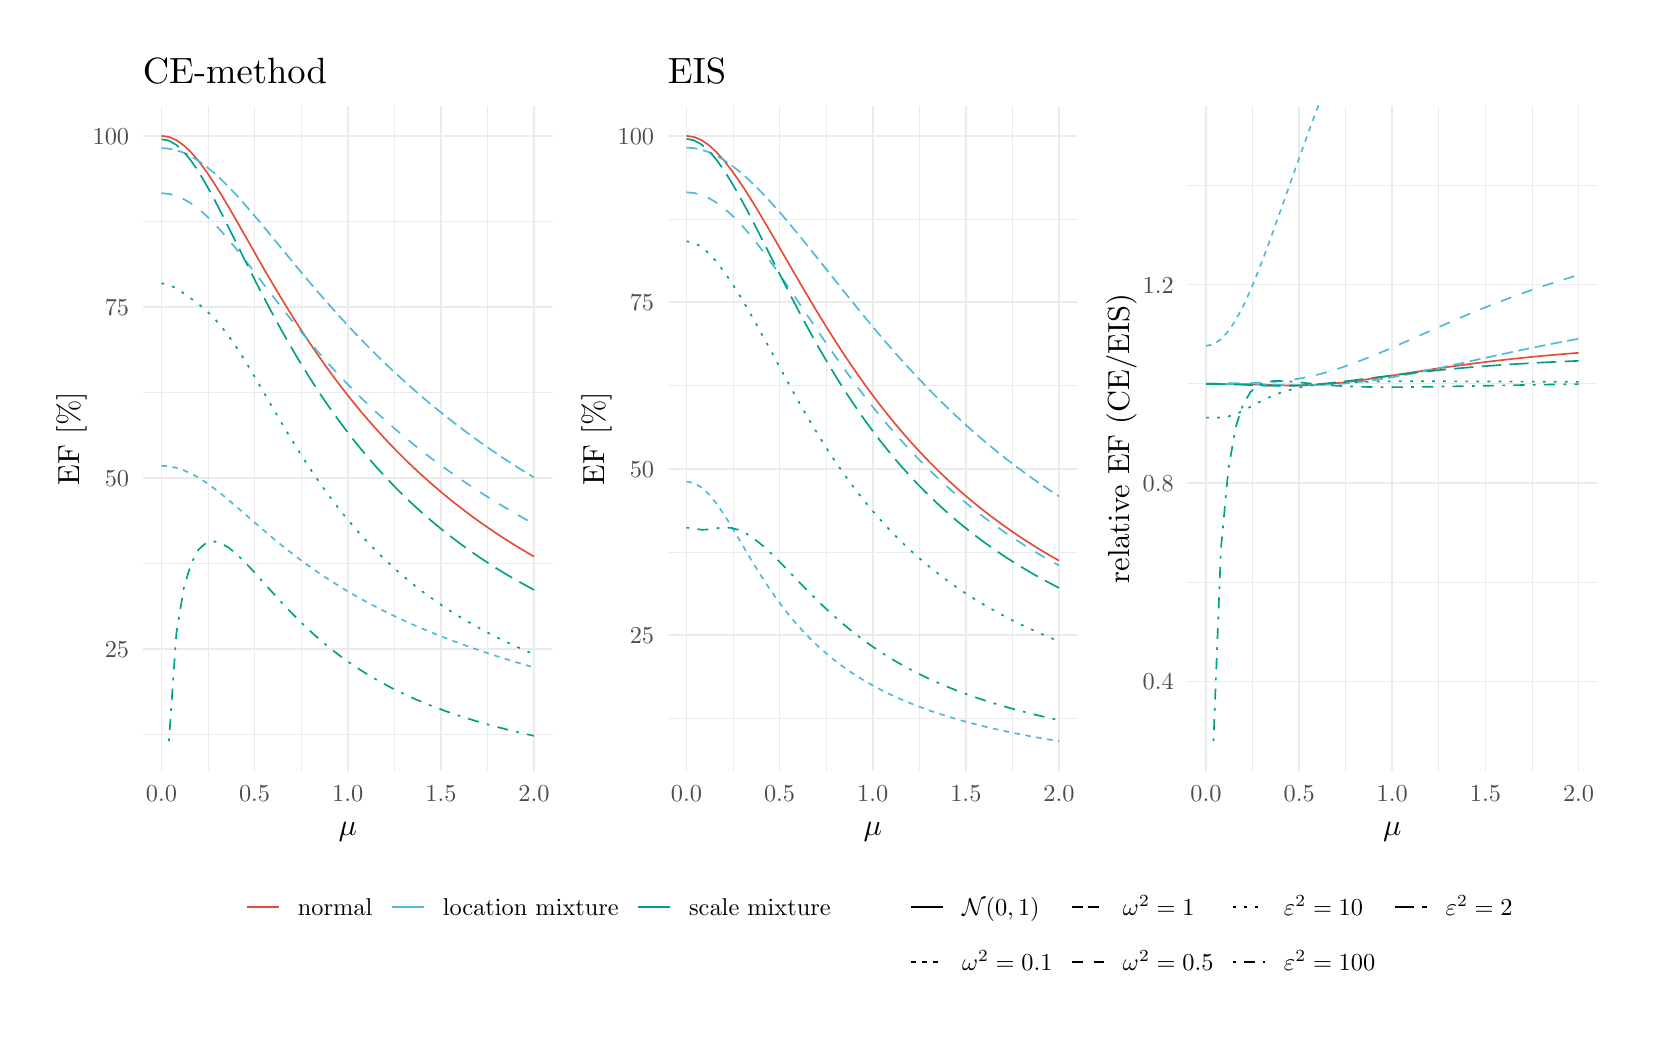
\begin{tikzpicture}[x=1pt,y=1pt]
\definecolor{fillColor}{RGB}{255,255,255}
\path[use as bounding box,fill=fillColor,fill opacity=0.00] (0,0) rectangle (578.16,361.35);
\begin{scope}
\path[clip] ( 41.61, 92.59) rectangle (189.71,333.19);
\definecolor{drawColor}{gray}{0.92}

\path[draw=drawColor,line width= 0.3pt,line join=round] ( 41.61,106.06) --
	(189.71,106.06);

\path[draw=drawColor,line width= 0.3pt,line join=round] ( 41.61,167.83) --
	(189.71,167.83);

\path[draw=drawColor,line width= 0.3pt,line join=round] ( 41.61,229.60) --
	(189.71,229.60);

\path[draw=drawColor,line width= 0.3pt,line join=round] ( 41.61,291.37) --
	(189.71,291.37);

\path[draw=drawColor,line width= 0.3pt,line join=round] ( 65.17, 92.59) --
	( 65.17,333.19);

\path[draw=drawColor,line width= 0.3pt,line join=round] ( 98.83, 92.59) --
	( 98.83,333.19);

\path[draw=drawColor,line width= 0.3pt,line join=round] (132.49, 92.59) --
	(132.49,333.19);

\path[draw=drawColor,line width= 0.3pt,line join=round] (166.14, 92.59) --
	(166.14,333.19);

\path[draw=drawColor,line width= 0.6pt,line join=round] ( 41.61,136.94) --
	(189.71,136.94);

\path[draw=drawColor,line width= 0.6pt,line join=round] ( 41.61,198.71) --
	(189.71,198.71);

\path[draw=drawColor,line width= 0.6pt,line join=round] ( 41.61,260.49) --
	(189.71,260.49);

\path[draw=drawColor,line width= 0.6pt,line join=round] ( 41.61,322.26) --
	(189.71,322.26);

\path[draw=drawColor,line width= 0.6pt,line join=round] ( 48.34, 92.59) --
	( 48.34,333.19);

\path[draw=drawColor,line width= 0.6pt,line join=round] ( 82.00, 92.59) --
	( 82.00,333.19);

\path[draw=drawColor,line width= 0.6pt,line join=round] (115.66, 92.59) --
	(115.66,333.19);

\path[draw=drawColor,line width= 0.6pt,line join=round] (149.32, 92.59) --
	(149.32,333.19);

\path[draw=drawColor,line width= 0.6pt,line join=round] (182.97, 92.59) --
	(182.97,333.19);
\definecolor{drawColor}{RGB}{230,75,53}

\path[draw=drawColor,line width= 0.6pt,line join=round] ( 48.34,322.26) --
	( 51.04,321.86) --
	( 53.73,320.70) --
	( 56.42,318.80) --
	( 59.11,316.24) --
	( 61.81,313.10) --
	( 64.50,309.47) --
	( 67.19,305.45) --
	( 69.88,301.14) --
	( 72.58,296.62) --
	( 75.27,291.96) --
	( 77.96,287.23) --
	( 80.65,282.47) --
	( 83.35,277.74) --
	( 86.04,273.05) --
	( 88.73,268.45) --
	( 91.42,263.93) --
	( 94.12,259.52) --
	( 96.81,255.22) --
	( 99.50,251.05) --
	(102.20,246.99) --
	(104.89,243.05) --
	(107.58,239.24) --
	(110.27,235.54) --
	(112.97,231.96) --
	(115.66,228.50) --
	(118.35,225.15) --
	(121.04,221.90) --
	(123.74,218.77) --
	(126.43,215.73) --
	(129.12,212.80) --
	(131.81,209.96) --
	(134.51,207.21) --
	(137.20,204.55) --
	(139.89,201.98) --
	(142.58,199.49) --
	(145.28,197.08) --
	(147.97,194.75) --
	(150.66,192.49) --
	(153.35,190.30) --
	(156.05,188.18) --
	(158.74,186.13) --
	(161.43,184.14) --
	(164.13,182.21) --
	(166.82,180.34) --
	(169.51,178.52) --
	(172.20,176.76) --
	(174.90,175.06) --
	(177.59,173.40) --
	(180.28,171.79) --
	(182.97,170.23);
\definecolor{drawColor}{RGB}{77,187,213}

\path[draw=drawColor,line width= 0.6pt,dash pattern=on 2pt off 2pt ,line join=round] ( 48.34,203.05) --
	( 51.04,202.86) --
	( 53.73,202.31) --
	( 56.42,201.41) --
	( 59.11,200.20) --
	( 61.81,198.70) --
	( 64.50,196.95) --
	( 67.19,195.01) --
	( 69.88,192.91) --
	( 72.58,190.69) --
	( 75.27,188.40) --
	( 77.96,186.07) --
	( 80.65,183.72) --
	( 83.35,181.39) --
	( 86.04,179.08) --
	( 88.73,176.81) --
	( 91.42,174.60) --
	( 94.12,172.45) --
	( 96.81,170.37) --
	( 99.50,168.36) --
	(102.20,166.41) --
	(104.89,164.54) --
	(107.58,162.73) --
	(110.27,160.98) --
	(112.97,159.30) --
	(115.66,157.68) --
	(118.35,156.12) --
	(121.04,154.61) --
	(123.74,153.16) --
	(126.43,151.75) --
	(129.12,150.39) --
	(131.81,149.08) --
	(134.51,147.80) --
	(137.20,146.57) --
	(139.89,145.37) --
	(142.58,144.21) --
	(145.28,143.08) --
	(147.97,141.99) --
	(150.66,140.93) --
	(153.35,139.89) --
	(156.05,138.89) --
	(158.74,137.91) --
	(161.43,136.96) --
	(164.13,136.03) --
	(166.82,135.13) --
	(169.51,134.25) --
	(172.20,133.39) --
	(174.90,132.55) --
	(177.59,131.74) --
	(180.28,130.94) --
	(182.97,130.16);

\path[draw=drawColor,line width= 0.6pt,dash pattern=on 4pt off 2pt ,line join=round] ( 48.34,317.84) --
	( 51.04,317.65) --
	( 53.73,317.07) --
	( 56.42,316.12) --
	( 59.11,314.81) --
	( 61.81,313.17) --
	( 64.50,311.22) --
	( 67.19,309.00) --
	( 69.88,306.53) --
	( 72.58,303.86) --
	( 75.27,301.02) --
	( 77.96,298.03) --
	( 80.65,294.93) --
	( 83.35,291.75) --
	( 86.04,288.52) --
	( 88.73,285.25) --
	( 91.42,281.96) --
	( 94.12,278.68) --
	( 96.81,275.42) --
	( 99.50,272.18) --
	(102.20,268.99) --
	(104.89,265.83) --
	(107.58,262.73) --
	(110.27,259.69) --
	(112.97,256.70) --
	(115.66,253.78) --
	(118.35,250.91) --
	(121.04,248.11) --
	(123.74,245.37) --
	(126.43,242.70) --
	(129.12,240.08) --
	(131.81,237.53) --
	(134.51,235.03) --
	(137.20,232.60) --
	(139.89,230.22) --
	(142.58,227.89) --
	(145.28,225.62) --
	(147.97,223.41) --
	(150.66,221.24) --
	(153.35,219.13) --
	(156.05,217.06) --
	(158.74,215.04) --
	(161.43,213.06) --
	(164.13,211.13) --
	(166.82,209.25) --
	(169.51,207.40) --
	(172.20,205.60) --
	(174.90,203.84) --
	(177.59,202.11) --
	(180.28,200.43) --
	(182.97,198.78);

\path[draw=drawColor,line width= 0.6pt,dash pattern=on 4pt off 4pt ,line join=round] ( 48.34,301.53) --
	( 51.04,301.29) --
	( 53.73,300.57) --
	( 56.42,299.40) --
	( 59.11,297.79) --
	( 61.81,295.79) --
	( 64.50,293.45) --
	( 67.19,290.79) --
	( 69.88,287.89) --
	( 72.58,284.77) --
	( 75.27,281.50) --
	( 77.96,278.12) --
	( 80.65,274.66) --
	( 83.35,271.15) --
	( 86.04,267.64) --
	( 88.73,264.13) --
	( 91.42,260.66) --
	( 94.12,257.24) --
	( 96.81,253.87) --
	( 99.50,250.58) --
	(102.20,247.35) --
	(104.89,244.21) --
	(107.58,241.15) --
	(110.27,238.17) --
	(112.97,235.27) --
	(115.66,232.46) --
	(118.35,229.72) --
	(121.04,227.06) --
	(123.74,224.47) --
	(126.43,221.96) --
	(129.12,219.52) --
	(131.81,217.15) --
	(134.51,214.84) --
	(137.20,212.59) --
	(139.89,210.40) --
	(142.58,208.27) --
	(145.28,206.20) --
	(147.97,204.18) --
	(150.66,202.22) --
	(153.35,200.30) --
	(156.05,198.43) --
	(158.74,196.61) --
	(161.43,194.83) --
	(164.13,193.10) --
	(166.82,191.40) --
	(169.51,189.75) --
	(172.20,188.14) --
	(174.90,186.56) --
	(177.59,185.03) --
	(180.28,183.52) --
	(182.97,182.06);
\definecolor{drawColor}{RGB}{0,160,135}

\path[draw=drawColor,line width= 0.6pt,dash pattern=on 1pt off 3pt ,line join=round] ( 48.34,268.97) --
	( 51.04,268.46) --
	( 53.73,267.10) --
	( 56.42,265.33) --
	( 59.11,263.43) --
	( 61.81,261.42) --
	( 64.50,259.16) --
	( 67.19,256.55) --
	( 69.88,253.49) --
	( 72.58,250.01) --
	( 75.27,246.13) --
	( 77.96,241.94) --
	( 80.65,237.52) --
	( 83.35,232.96) --
	( 86.04,228.32) --
	( 88.73,223.68) --
	( 91.42,219.08) --
	( 94.12,214.56) --
	( 96.81,210.16) --
	( 99.50,205.89) --
	(102.20,201.77) --
	(104.89,197.81) --
	(107.58,194.01) --
	(110.27,190.37) --
	(112.97,186.89) --
	(115.66,183.56) --
	(118.35,180.39) --
	(121.04,177.37) --
	(123.74,174.48) --
	(126.43,171.73) --
	(129.12,169.10) --
	(131.81,166.60) --
	(134.51,164.20) --
	(137.20,161.92) --
	(139.89,159.74) --
	(142.58,157.66) --
	(145.28,155.66) --
	(147.97,153.75) --
	(150.66,151.93) --
	(153.35,150.18) --
	(156.05,148.50) --
	(158.74,146.89) --
	(161.43,145.35) --
	(164.13,143.87) --
	(166.82,142.44) --
	(169.51,141.07) --
	(172.20,139.75) --
	(174.90,138.48) --
	(177.59,137.26) --
	(180.28,136.08) --
	(182.97,134.95);

\path[draw=drawColor,line width= 0.6pt,dash pattern=on 1pt off 3pt on 4pt off 3pt ,line join=round] ( 51.04,103.53) --
	( 53.73,142.49) --
	( 56.42,158.90) --
	( 59.11,167.90) --
	( 61.81,172.83) --
	( 64.50,175.17) --
	( 67.19,175.73) --
	( 69.88,175.04) --
	( 72.58,173.48) --
	( 75.27,171.31) --
	( 77.96,168.74) --
	( 80.65,165.93) --
	( 83.35,162.97) --
	( 86.04,159.96) --
	( 88.73,156.97) --
	( 91.42,154.02) --
	( 94.12,151.16) --
	( 96.81,148.39) --
	( 99.50,145.74) --
	(102.20,143.21) --
	(104.89,140.80) --
	(107.58,138.51) --
	(110.27,136.34) --
	(112.97,134.28) --
	(115.66,132.33) --
	(118.35,130.48) --
	(121.04,128.74) --
	(123.74,127.08) --
	(126.43,125.52) --
	(129.12,124.03) --
	(131.81,122.62) --
	(134.51,121.28) --
	(137.20,120.01) --
	(139.89,118.80) --
	(142.58,117.66) --
	(145.28,116.56) --
	(147.97,115.52) --
	(150.66,114.52) --
	(153.35,113.58) --
	(156.05,112.67) --
	(158.74,111.80) --
	(161.43,110.97) --
	(164.13,110.18) --
	(166.82,109.42) --
	(169.51,108.69) --
	(172.20,107.99) --
	(174.90,107.32) --
	(177.59,106.67) --
	(180.28,106.05) --
	(182.97,105.45);

\path[draw=drawColor,line width= 0.6pt,dash pattern=on 7pt off 3pt ,line join=round] ( 48.34,321.06) --
	( 51.04,320.54) --
	( 53.73,318.99) --
	( 56.42,316.50) --
	( 59.11,313.18) --
	( 61.81,309.19) --
	( 64.50,304.66) --
	( 67.19,299.75) --
	( 69.88,294.57) --
	( 72.58,289.23) --
	( 75.27,283.81) --
	( 77.96,278.39) --
	( 80.65,273.02) --
	( 83.35,267.72) --
	( 86.04,262.53) --
	( 88.73,257.47) --
	( 91.42,252.55) --
	( 94.12,247.78) --
	( 96.81,243.16) --
	( 99.50,238.69) --
	(102.20,234.38) --
	(104.89,230.23) --
	(107.58,226.22) --
	(110.27,222.37) --
	(112.97,218.66) --
	(115.66,215.08) --
	(118.35,211.65) --
	(121.04,208.34) --
	(123.74,205.16) --
	(126.43,202.10) --
	(129.12,199.15) --
	(131.81,196.32) --
	(134.51,193.59) --
	(137.20,190.96) --
	(139.89,188.43) --
	(142.58,186.00) --
	(145.28,183.65) --
	(147.97,181.39) --
	(150.66,179.21) --
	(153.35,177.10) --
	(156.05,175.07) --
	(158.74,173.11) --
	(161.43,171.22) --
	(164.13,169.39) --
	(166.82,167.63) --
	(169.51,165.92) --
	(172.20,164.27) --
	(174.90,162.67) --
	(177.59,161.13) --
	(180.28,159.64) --
	(182.97,158.19);
\end{scope}
\begin{scope}
\path[clip] (  0.00,  0.00) rectangle (578.16,361.35);
\definecolor{drawColor}{gray}{0.30}

\node[text=drawColor,anchor=base east,inner sep=0pt, outer sep=0pt, scale=  0.88] at ( 36.66,133.91) {25};

\node[text=drawColor,anchor=base east,inner sep=0pt, outer sep=0pt, scale=  0.88] at ( 36.66,195.68) {50};

\node[text=drawColor,anchor=base east,inner sep=0pt, outer sep=0pt, scale=  0.88] at ( 36.66,257.46) {75};

\node[text=drawColor,anchor=base east,inner sep=0pt, outer sep=0pt, scale=  0.88] at ( 36.66,319.23) {100};
\end{scope}
\begin{scope}
\path[clip] (  0.00,  0.00) rectangle (578.16,361.35);
\definecolor{drawColor}{gray}{0.30}

\node[text=drawColor,anchor=base,inner sep=0pt, outer sep=0pt, scale=  0.88] at ( 48.34, 81.58) {0.0};

\node[text=drawColor,anchor=base,inner sep=0pt, outer sep=0pt, scale=  0.88] at ( 82.00, 81.58) {0.5};

\node[text=drawColor,anchor=base,inner sep=0pt, outer sep=0pt, scale=  0.88] at (115.66, 81.58) {1.0};

\node[text=drawColor,anchor=base,inner sep=0pt, outer sep=0pt, scale=  0.88] at (149.32, 81.58) {1.5};

\node[text=drawColor,anchor=base,inner sep=0pt, outer sep=0pt, scale=  0.88] at (182.97, 81.58) {2.0};
\end{scope}
\begin{scope}
\path[clip] (  0.00,  0.00) rectangle (578.16,361.35);
\definecolor{drawColor}{RGB}{0,0,0}

\node[text=drawColor,anchor=base,inner sep=0pt, outer sep=0pt, scale=  1.10] at (115.66, 69.55) {$\mu$};
\end{scope}
\begin{scope}
\path[clip] (  0.00,  0.00) rectangle (578.16,361.35);
\definecolor{drawColor}{RGB}{0,0,0}

\node[text=drawColor,rotate= 90.00,anchor=base,inner sep=0pt, outer sep=0pt, scale=  1.10] at ( 18.58,212.89) {EF [\%]};
\end{scope}
\begin{scope}
\path[clip] (  0.00,  0.00) rectangle (578.16,361.35);
\definecolor{drawColor}{RGB}{0,0,0}

\node[text=drawColor,anchor=base west,inner sep=0pt, outer sep=0pt, scale=  1.32] at ( 41.61,341.26) {CE-method};
\end{scope}
\begin{scope}
\path[clip] (231.32, 92.59) rectangle (379.41,333.19);
\definecolor{drawColor}{gray}{0.92}

\path[draw=drawColor,line width= 0.3pt,line join=round] (231.32,111.72) --
	(379.41,111.72);

\path[draw=drawColor,line width= 0.3pt,line join=round] (231.32,171.87) --
	(379.41,171.87);

\path[draw=drawColor,line width= 0.3pt,line join=round] (231.32,232.03) --
	(379.41,232.03);

\path[draw=drawColor,line width= 0.3pt,line join=round] (231.32,292.18) --
	(379.41,292.18);

\path[draw=drawColor,line width= 0.3pt,line join=round] (254.88, 92.59) --
	(254.88,333.19);

\path[draw=drawColor,line width= 0.3pt,line join=round] (288.53, 92.59) --
	(288.53,333.19);

\path[draw=drawColor,line width= 0.3pt,line join=round] (322.19, 92.59) --
	(322.19,333.19);

\path[draw=drawColor,line width= 0.3pt,line join=round] (355.85, 92.59) --
	(355.85,333.19);

\path[draw=drawColor,line width= 0.6pt,line join=round] (231.32,141.80) --
	(379.41,141.80);

\path[draw=drawColor,line width= 0.6pt,line join=round] (231.32,201.95) --
	(379.41,201.95);

\path[draw=drawColor,line width= 0.6pt,line join=round] (231.32,262.10) --
	(379.41,262.10);

\path[draw=drawColor,line width= 0.6pt,line join=round] (231.32,322.26) --
	(379.41,322.26);

\path[draw=drawColor,line width= 0.6pt,line join=round] (238.05, 92.59) --
	(238.05,333.19);

\path[draw=drawColor,line width= 0.6pt,line join=round] (271.71, 92.59) --
	(271.71,333.19);

\path[draw=drawColor,line width= 0.6pt,line join=round] (305.36, 92.59) --
	(305.36,333.19);

\path[draw=drawColor,line width= 0.6pt,line join=round] (339.02, 92.59) --
	(339.02,333.19);

\path[draw=drawColor,line width= 0.6pt,line join=round] (372.68, 92.59) --
	(372.68,333.19);
\definecolor{drawColor}{RGB}{230,75,53}

\path[draw=drawColor,line width= 0.6pt,line join=round] (238.05,322.26) --
	(240.74,321.87) --
	(243.43,320.74) --
	(246.13,318.91) --
	(248.82,316.45) --
	(251.51,313.46) --
	(254.20,310.02) --
	(256.90,306.22) --
	(259.59,302.14) --
	(262.28,297.84) --
	(264.97,293.38) --
	(267.67,288.81) --
	(270.36,284.17) --
	(273.05,279.50) --
	(275.74,274.83) --
	(278.44,270.19) --
	(281.13,265.59) --
	(283.82,261.06) --
	(286.51,256.61) --
	(289.21,252.25) --
	(291.90,248.00) --
	(294.59,243.86) --
	(297.29,239.83) --
	(299.98,235.92) --
	(302.67,232.14) --
	(305.36,228.48) --
	(308.06,224.93) --
	(310.75,221.51) --
	(313.44,218.21) --
	(316.13,215.02) --
	(318.83,211.94) --
	(321.52,208.98) --
	(324.21,206.12) --
	(326.90,203.36) --
	(329.60,200.70) --
	(332.29,198.13) --
	(334.98,195.66) --
	(337.67,193.27) --
	(340.37,190.97) --
	(343.06,188.75) --
	(345.75,186.61) --
	(348.44,184.54) --
	(351.14,182.54) --
	(353.83,180.61) --
	(356.52,178.74) --
	(359.22,176.94) --
	(361.91,175.19) --
	(364.60,173.50) --
	(367.29,171.87) --
	(369.99,170.29) --
	(372.68,168.76);
\definecolor{drawColor}{RGB}{77,187,213}

\path[draw=drawColor,line width= 0.6pt,dash pattern=on 2pt off 2pt ,line join=round] (238.05,197.32) --
	(240.74,196.79) --
	(243.43,195.24) --
	(246.13,192.76) --
	(248.82,189.49) --
	(251.51,185.59) --
	(254.20,181.29) --
	(256.90,176.77) --
	(259.59,172.19) --
	(262.28,167.70) --
	(264.97,163.36) --
	(267.67,159.23) --
	(270.36,155.34) --
	(273.05,151.70) --
	(275.74,148.31) --
	(278.44,145.15) --
	(281.13,142.23) --
	(283.82,139.52) --
	(286.51,137.00) --
	(289.21,134.66) --
	(291.90,132.49) --
	(294.59,130.47) --
	(297.29,128.59) --
	(299.98,126.84) --
	(302.67,125.20) --
	(305.36,123.66) --
	(308.06,122.22) --
	(310.75,120.87) --
	(313.44,119.61) --
	(316.13,118.41) --
	(318.83,117.29) --
	(321.52,116.23) --
	(324.21,115.22) --
	(326.90,114.27) --
	(329.60,113.37) --
	(332.29,112.52) --
	(334.98,111.70) --
	(337.67,110.93) --
	(340.37,110.20) --
	(343.06,109.50) --
	(345.75,108.83) --
	(348.44,108.19) --
	(351.14,107.58) --
	(353.83,107.00) --
	(356.52,106.44) --
	(359.22,105.90) --
	(361.91,105.39) --
	(364.60,104.90) --
	(367.29,104.42) --
	(369.99,103.97) --
	(372.68,103.53);

\path[draw=drawColor,line width= 0.6pt,dash pattern=on 4pt off 2pt ,line join=round] (238.05,318.00) --
	(240.74,317.81) --
	(243.43,317.26) --
	(246.13,316.35) --
	(248.82,315.11) --
	(251.51,313.55) --
	(254.20,311.71) --
	(256.90,309.61) --
	(259.59,307.28) --
	(262.28,304.75) --
	(264.97,302.05) --
	(267.67,299.19) --
	(270.36,296.21) --
	(273.05,293.11) --
	(275.74,289.93) --
	(278.44,286.67) --
	(281.13,283.37) --
	(283.82,280.02) --
	(286.51,276.64) --
	(289.21,273.26) --
	(291.90,269.87) --
	(294.59,266.50) --
	(297.29,263.14) --
	(299.98,259.82) --
	(302.67,256.53) --
	(305.36,253.29) --
	(308.06,250.10) --
	(310.75,246.96) --
	(313.44,243.87) --
	(316.13,240.85) --
	(318.83,237.89) --
	(321.52,234.99) --
	(324.21,232.17) --
	(326.90,229.40) --
	(329.60,226.71) --
	(332.29,224.08) --
	(334.98,221.51) --
	(337.67,219.01) --
	(340.37,216.58) --
	(343.06,214.21) --
	(345.75,211.90) --
	(348.44,209.66) --
	(351.14,207.47) --
	(353.83,205.35) --
	(356.52,203.28) --
	(359.22,201.27) --
	(361.91,199.31) --
	(364.60,197.40) --
	(367.29,195.54) --
	(369.99,193.74) --
	(372.68,191.98);

\path[draw=drawColor,line width= 0.6pt,dash pattern=on 4pt off 4pt ,line join=round] (238.05,301.87) --
	(240.74,301.63) --
	(243.43,300.92) --
	(246.13,299.76) --
	(248.82,298.17) --
	(251.51,296.18) --
	(254.20,293.83) --
	(256.90,291.15) --
	(259.59,288.17) --
	(262.28,284.94) --
	(264.97,281.49) --
	(267.67,277.87) --
	(270.36,274.10) --
	(273.05,270.23) --
	(275.74,266.28) --
	(278.44,262.28) --
	(281.13,258.27) --
	(283.82,254.26) --
	(286.51,250.28) --
	(289.21,246.35) --
	(291.90,242.48) --
	(294.59,238.68) --
	(297.29,234.96) --
	(299.98,231.33) --
	(302.67,227.80) --
	(305.36,224.37) --
	(308.06,221.03) --
	(310.75,217.80) --
	(313.44,214.66) --
	(316.13,211.63) --
	(318.83,208.70) --
	(321.52,205.87) --
	(324.21,203.13) --
	(326.90,200.48) --
	(329.60,197.92) --
	(332.29,195.46) --
	(334.98,193.07) --
	(337.67,190.77) --
	(340.37,188.55) --
	(343.06,186.40) --
	(345.75,184.32) --
	(348.44,182.32) --
	(351.14,180.38) --
	(353.83,178.51) --
	(356.52,176.70) --
	(359.22,174.94) --
	(361.91,173.25) --
	(364.60,171.61) --
	(367.29,170.02) --
	(369.99,168.48) --
	(372.68,166.99);
\definecolor{drawColor}{RGB}{0,160,135}

\path[draw=drawColor,line width= 0.6pt,dash pattern=on 1pt off 3pt ,line join=round] (238.05,284.15) --
	(240.74,283.65) --
	(243.43,282.16) --
	(246.13,279.84) --
	(248.82,276.85) --
	(251.51,273.35) --
	(254.20,269.45) --
	(256.90,265.22) --
	(259.59,260.72) --
	(262.28,256.02) --
	(264.97,251.16) --
	(267.67,246.21) --
	(270.36,241.22) --
	(273.05,236.25) --
	(275.74,231.32) --
	(278.44,226.49) --
	(281.13,221.78) --
	(283.82,217.21) --
	(286.51,212.80) --
	(289.21,208.56) --
	(291.90,204.48) --
	(294.59,200.58) --
	(297.29,196.86) --
	(299.98,193.30) --
	(302.67,189.90) --
	(305.36,186.67) --
	(308.06,183.59) --
	(310.75,180.65) --
	(313.44,177.85) --
	(316.13,175.18) --
	(318.83,172.64) --
	(321.52,170.21) --
	(324.21,167.90) --
	(326.90,165.69) --
	(329.60,163.58) --
	(332.29,161.57) --
	(334.98,159.64) --
	(337.67,157.80) --
	(340.37,156.03) --
	(343.06,154.34) --
	(345.75,152.72) --
	(348.44,151.17) --
	(351.14,149.67) --
	(353.83,148.24) --
	(356.52,146.86) --
	(359.22,145.54) --
	(361.91,144.26) --
	(364.60,143.04) --
	(367.29,141.86) --
	(369.99,140.72) --
	(372.68,139.62);

\path[draw=drawColor,line width= 0.6pt,dash pattern=on 1pt off 3pt on 4pt off 3pt ,line join=round] (238.05,180.67) --
	(240.74,180.39) --
	(243.43,179.92) --
	(246.13,180.02) --
	(248.82,180.46) --
	(251.51,180.75) --
	(254.20,180.59) --
	(256.90,179.87) --
	(259.59,178.59) --
	(262.28,176.84) --
	(264.97,174.71) --
	(267.67,172.30) --
	(270.36,169.68) --
	(273.05,166.95) --
	(275.74,164.16) --
	(278.44,161.36) --
	(281.13,158.59) --
	(283.82,155.87) --
	(286.51,153.24) --
	(289.21,150.70) --
	(291.90,148.26) --
	(294.59,145.93) --
	(297.29,143.71) --
	(299.98,141.59) --
	(302.67,139.58) --
	(305.36,137.67) --
	(308.06,135.86) --
	(310.75,134.14) --
	(313.44,132.51) --
	(316.13,130.97) --
	(318.83,129.50) --
	(321.52,128.11) --
	(324.21,126.79) --
	(326.90,125.53) --
	(329.60,124.34) --
	(332.29,123.20) --
	(334.98,122.12) --
	(337.67,121.09) --
	(340.37,120.10) --
	(343.06,119.17) --
	(345.75,118.27) --
	(348.44,117.41) --
	(351.14,116.59) --
	(353.83,115.81) --
	(356.52,115.06) --
	(359.22,114.34) --
	(361.91,113.65) --
	(364.60,112.98) --
	(367.29,112.35) --
	(369.99,111.73) --
	(372.68,111.14);

\path[draw=drawColor,line width= 0.6pt,dash pattern=on 7pt off 3pt ,line join=round] (238.05,321.16) --
	(240.74,320.66) --
	(243.43,319.19) --
	(246.13,316.83) --
	(248.82,313.70) --
	(251.51,309.94) --
	(254.20,305.67) --
	(256.90,301.02) --
	(259.59,296.07) --
	(262.28,290.94) --
	(264.97,285.67) --
	(267.67,280.34) --
	(270.36,275.00) --
	(273.05,269.69) --
	(275.74,264.45) --
	(278.44,259.30) --
	(281.13,254.26) --
	(283.82,249.35) --
	(286.51,244.59) --
	(289.21,239.97) --
	(291.90,235.52) --
	(294.59,231.22) --
	(297.29,227.08) --
	(299.98,223.10) --
	(302.67,219.28) --
	(305.36,215.60) --
	(308.06,212.08) --
	(310.75,208.70) --
	(313.44,205.45) --
	(316.13,202.34) --
	(318.83,199.35) --
	(321.52,196.49) --
	(324.21,193.74) --
	(326.90,191.10) --
	(329.60,188.57) --
	(332.29,186.14) --
	(334.98,183.80) --
	(337.67,181.56) --
	(340.37,179.40) --
	(343.06,177.32) --
	(345.75,175.32) --
	(348.44,173.40) --
	(351.14,171.55) --
	(353.83,169.76) --
	(356.52,168.04) --
	(359.22,166.38) --
	(361.91,164.78) --
	(364.60,163.23) --
	(367.29,161.74) --
	(369.99,160.29) --
	(372.68,158.90);
\end{scope}
\begin{scope}
\path[clip] (  0.00,  0.00) rectangle (578.16,361.35);
\definecolor{drawColor}{gray}{0.30}

\node[text=drawColor,anchor=base east,inner sep=0pt, outer sep=0pt, scale=  0.88] at (226.37,138.76) {25};

\node[text=drawColor,anchor=base east,inner sep=0pt, outer sep=0pt, scale=  0.88] at (226.37,198.92) {50};

\node[text=drawColor,anchor=base east,inner sep=0pt, outer sep=0pt, scale=  0.88] at (226.37,259.07) {75};

\node[text=drawColor,anchor=base east,inner sep=0pt, outer sep=0pt, scale=  0.88] at (226.37,319.23) {100};
\end{scope}
\begin{scope}
\path[clip] (  0.00,  0.00) rectangle (578.16,361.35);
\definecolor{drawColor}{gray}{0.30}

\node[text=drawColor,anchor=base,inner sep=0pt, outer sep=0pt, scale=  0.88] at (238.05, 81.58) {0.0};

\node[text=drawColor,anchor=base,inner sep=0pt, outer sep=0pt, scale=  0.88] at (271.71, 81.58) {0.5};

\node[text=drawColor,anchor=base,inner sep=0pt, outer sep=0pt, scale=  0.88] at (305.36, 81.58) {1.0};

\node[text=drawColor,anchor=base,inner sep=0pt, outer sep=0pt, scale=  0.88] at (339.02, 81.58) {1.5};

\node[text=drawColor,anchor=base,inner sep=0pt, outer sep=0pt, scale=  0.88] at (372.68, 81.58) {2.0};
\end{scope}
\begin{scope}
\path[clip] (  0.00,  0.00) rectangle (578.16,361.35);
\definecolor{drawColor}{RGB}{0,0,0}

\node[text=drawColor,anchor=base,inner sep=0pt, outer sep=0pt, scale=  1.10] at (305.36, 69.55) {$\mu$};
\end{scope}
\begin{scope}
\path[clip] (  0.00,  0.00) rectangle (578.16,361.35);
\definecolor{drawColor}{RGB}{0,0,0}

\node[text=drawColor,rotate= 90.00,anchor=base,inner sep=0pt, outer sep=0pt, scale=  1.10] at (208.28,212.89) {EF [\%]};
\end{scope}
\begin{scope}
\path[clip] (  0.00,  0.00) rectangle (578.16,361.35);
\definecolor{drawColor}{RGB}{0,0,0}

\node[text=drawColor,anchor=base west,inner sep=0pt, outer sep=0pt, scale=  1.32] at (231.32,341.26) {EIS};
\end{scope}
\begin{scope}
\path[clip] (419.07, 92.59) rectangle (567.16,333.19);
\definecolor{drawColor}{gray}{0.92}

\path[draw=drawColor,line width= 0.3pt,line join=round] (419.07,160.95) --
	(567.16,160.95);

\path[draw=drawColor,line width= 0.3pt,line join=round] (419.07,232.64) --
	(567.16,232.64);

\path[draw=drawColor,line width= 0.3pt,line join=round] (419.07,304.33) --
	(567.16,304.33);

\path[draw=drawColor,line width= 0.3pt,line join=round] (442.63, 92.59) --
	(442.63,333.19);

\path[draw=drawColor,line width= 0.3pt,line join=round] (476.28, 92.59) --
	(476.28,333.19);

\path[draw=drawColor,line width= 0.3pt,line join=round] (509.94, 92.59) --
	(509.94,333.19);

\path[draw=drawColor,line width= 0.3pt,line join=round] (543.60, 92.59) --
	(543.60,333.19);

\path[draw=drawColor,line width= 0.6pt,line join=round] (419.07,125.10) --
	(567.16,125.10);

\path[draw=drawColor,line width= 0.6pt,line join=round] (419.07,196.80) --
	(567.16,196.80);

\path[draw=drawColor,line width= 0.6pt,line join=round] (419.07,268.49) --
	(567.16,268.49);

\path[draw=drawColor,line width= 0.6pt,line join=round] (425.80, 92.59) --
	(425.80,333.19);

\path[draw=drawColor,line width= 0.6pt,line join=round] (459.46, 92.59) --
	(459.46,333.19);

\path[draw=drawColor,line width= 0.6pt,line join=round] (493.11, 92.59) --
	(493.11,333.19);

\path[draw=drawColor,line width= 0.6pt,line join=round] (526.77, 92.59) --
	(526.77,333.19);

\path[draw=drawColor,line width= 0.6pt,line join=round] (560.43, 92.59) --
	(560.43,333.19);
\definecolor{drawColor}{RGB}{230,75,53}

\path[draw=drawColor,line width= 0.6pt,line join=round] (425.80,232.64) --
	(428.49,232.64) --
	(431.18,232.64) --
	(433.88,232.63) --
	(436.57,232.60) --
	(439.26,232.54) --
	(441.95,232.47) --
	(444.65,232.38) --
	(447.34,232.28) --
	(450.03,232.19) --
	(452.72,232.11) --
	(455.42,232.06) --
	(458.11,232.06) --
	(460.80,232.10) --
	(463.49,232.19) --
	(466.19,232.33) --
	(468.88,232.52) --
	(471.57,232.75) --
	(474.26,233.02) --
	(476.96,233.34) --
	(479.65,233.68) --
	(482.34,234.04) --
	(485.04,234.43) --
	(487.73,234.83) --
	(490.42,235.24) --
	(493.11,235.66) --
	(495.81,236.09) --
	(498.50,236.51) --
	(501.19,236.93) --
	(503.88,237.34) --
	(506.58,237.75) --
	(509.27,238.16) --
	(511.96,238.55) --
	(514.65,238.93) --
	(517.35,239.31) --
	(520.04,239.67) --
	(522.73,240.02) --
	(525.42,240.37) --
	(528.12,240.70) --
	(530.81,241.01) --
	(533.50,241.32) --
	(536.19,241.62) --
	(538.89,241.91) --
	(541.58,242.18) --
	(544.27,242.45) --
	(546.97,242.70) --
	(549.66,242.95) --
	(552.35,243.19) --
	(555.04,243.42) --
	(557.74,243.64) --
	(560.43,243.85);
\definecolor{drawColor}{RGB}{77,187,213}

\path[draw=drawColor,line width= 0.6pt,dash pattern=on 2pt off 2pt ,line join=round] (425.80,246.35) --
	(428.49,246.96) --
	(431.18,248.75) --
	(433.88,251.69) --
	(436.57,255.75) --
	(439.26,260.81) --
	(441.95,266.72) --
	(444.65,273.29) --
	(447.34,280.34) --
	(450.03,287.72) --
	(452.72,295.27) --
	(455.42,302.89) --
	(458.11,310.50) --
	(460.80,318.03) --
	(463.49,325.45) --
	(466.19,332.73) --
	(468.88,339.84) --
	(471.57,346.79) --
	(474.26,353.56) --
	(476.96,360.15) --
	(479.65,366.57) --
	(482.34,372.82) --
	(485.04,378.89) --
	(487.73,384.80) --
	(490.42,390.55) --
	(493.11,396.13) --
	(495.81,401.55) --
	(498.50,406.82) --
	(501.19,411.93) --
	(503.88,416.89) --
	(506.58,421.71) --
	(509.27,426.38) --
	(511.96,430.91) --
	(514.65,435.30) --
	(517.35,439.56) --
	(520.04,443.68) --
	(522.73,447.67) --
	(525.42,451.54) --
	(528.12,455.29) --
	(530.81,458.92) --
	(533.50,462.43) --
	(536.19,465.82) --
	(538.89,469.11) --
	(541.58,472.30) --
	(544.27,475.38) --
	(546.97,478.36) --
	(549.66,481.25) --
	(552.35,484.04) --
	(555.04,486.75) --
	(557.74,489.36) --
	(560.43,491.90);

\path[draw=drawColor,line width= 0.6pt,dash pattern=on 4pt off 2pt ,line join=round] (425.80,232.61) --
	(428.49,232.61) --
	(431.18,232.60) --
	(433.88,232.59) --
	(436.57,232.56) --
	(439.26,232.53) --
	(441.95,232.49) --
	(444.65,232.43) --
	(447.34,232.37) --
	(450.03,232.31) --
	(452.72,232.25) --
	(455.42,232.20) --
	(458.11,232.17) --
	(460.80,232.16) --
	(463.49,232.19) --
	(466.19,232.24) --
	(468.88,232.33) --
	(471.57,232.47) --
	(474.26,232.64) --
	(476.96,232.86) --
	(479.65,233.13) --
	(482.34,233.43) --
	(485.04,233.78) --
	(487.73,234.16) --
	(490.42,234.58) --
	(493.11,235.02) --
	(495.81,235.50) --
	(498.50,236.00) --
	(501.19,236.53) --
	(503.88,237.07) --
	(506.58,237.63) --
	(509.27,238.20) --
	(511.96,238.78) --
	(514.65,239.37) --
	(517.35,239.96) --
	(520.04,240.56) --
	(522.73,241.15) --
	(525.42,241.75) --
	(528.12,242.34) --
	(530.81,242.94) --
	(533.50,243.52) --
	(536.19,244.10) --
	(538.89,244.67) --
	(541.58,245.24) --
	(544.27,245.80) --
	(546.97,246.34) --
	(549.66,246.88) --
	(552.35,247.41) --
	(555.04,247.93) --
	(557.74,248.44) --
	(560.43,248.93);

\path[draw=drawColor,line width= 0.6pt,dash pattern=on 4pt off 4pt ,line join=round] (425.80,232.81) --
	(428.49,232.81) --
	(431.18,232.82) --
	(433.88,232.83) --
	(436.57,232.86) --
	(439.26,232.90) --
	(441.95,232.95) --
	(444.65,233.04) --
	(447.34,233.18) --
	(450.03,233.36) --
	(452.72,233.61) --
	(455.42,233.92) --
	(458.11,234.32) --
	(460.80,234.79) --
	(463.49,235.35) --
	(466.19,235.99) --
	(468.88,236.71) --
	(471.57,237.50) --
	(474.26,238.36) --
	(476.96,239.28) --
	(479.65,240.26) --
	(482.34,241.29) --
	(485.04,242.36) --
	(487.73,243.46) --
	(490.42,244.60) --
	(493.11,245.75) --
	(495.81,246.93) --
	(498.50,248.12) --
	(501.19,249.31) --
	(503.88,250.50) --
	(506.58,251.70) --
	(509.27,252.89) --
	(511.96,254.07) --
	(514.65,255.23) --
	(517.35,256.39) --
	(520.04,257.53) --
	(522.73,258.65) --
	(525.42,259.75) --
	(528.12,260.83) --
	(530.81,261.88) --
	(533.50,262.92) --
	(536.19,263.93) --
	(538.89,264.92) --
	(541.58,265.89) --
	(544.27,266.83) --
	(546.97,267.75) --
	(549.66,268.64) --
	(552.35,269.52) --
	(555.04,270.36) --
	(557.74,271.19) --
	(560.43,271.99);
\definecolor{drawColor}{RGB}{0,160,135}

\path[draw=drawColor,line width= 0.6pt,dash pattern=on 1pt off 3pt ,line join=round] (425.80,220.44) --
	(428.49,220.42) --
	(431.18,220.47) --
	(433.88,220.87) --
	(436.57,221.73) --
	(439.26,222.97) --
	(441.95,224.40) --
	(444.65,225.85) --
	(447.34,227.21) --
	(450.03,228.41) --
	(452.72,229.43) --
	(455.42,230.28) --
	(458.11,230.97) --
	(460.80,231.54) --
	(463.49,231.99) --
	(466.19,232.35) --
	(468.88,232.64) --
	(471.57,232.86) --
	(474.26,233.04) --
	(476.96,233.18) --
	(479.65,233.29) --
	(482.34,233.37) --
	(485.04,233.43) --
	(487.73,233.48) --
	(490.42,233.52) --
	(493.11,233.54) --
	(495.81,233.56) --
	(498.50,233.57) --
	(501.19,233.57) --
	(503.88,233.57) --
	(506.58,233.57) --
	(509.27,233.57) --
	(511.96,233.56) --
	(514.65,233.55) --
	(517.35,233.54) --
	(520.04,233.53) --
	(522.73,233.52) --
	(525.42,233.51) --
	(528.12,233.50) --
	(530.81,233.49) --
	(533.50,233.47) --
	(536.19,233.46) --
	(538.89,233.45) --
	(541.58,233.44) --
	(544.27,233.43) --
	(546.97,233.41) --
	(549.66,233.40) --
	(552.35,233.39) --
	(555.04,233.38) --
	(557.74,233.37) --
	(560.43,233.36);

\path[draw=drawColor,line width= 0.6pt,dash pattern=on 1pt off 3pt on 4pt off 3pt ,line join=round] (428.49,103.53) --
	(431.18,172.96) --
	(433.88,201.96) --
	(436.57,217.19) --
	(439.26,225.40) --
	(441.95,229.80) --
	(444.65,232.09) --
	(447.34,233.20) --
	(450.03,233.64) --
	(452.72,233.70) --
	(455.42,233.56) --
	(458.11,233.32) --
	(460.80,233.04) --
	(463.49,232.76) --
	(466.19,232.50) --
	(468.88,232.27) --
	(471.57,232.06) --
	(474.26,231.89) --
	(476.96,231.76) --
	(479.65,231.65) --
	(482.34,231.57) --
	(485.04,231.51) --
	(487.73,231.48) --
	(490.42,231.46) --
	(493.11,231.46) --
	(495.81,231.47) --
	(498.50,231.48) --
	(501.19,231.51) --
	(503.88,231.55) --
	(506.58,231.58) --
	(509.27,231.63) --
	(511.96,231.67) --
	(514.65,231.72) --
	(517.35,231.77) --
	(520.04,231.83) --
	(522.73,231.88) --
	(525.42,231.93) --
	(528.12,231.98) --
	(530.81,232.03) --
	(533.50,232.09) --
	(536.19,232.14) --
	(538.89,232.19) --
	(541.58,232.24) --
	(544.27,232.28) --
	(546.97,232.33) --
	(549.66,232.38) --
	(552.35,232.42) --
	(555.04,232.46) --
	(557.74,232.51) --
	(560.43,232.55);

\path[draw=drawColor,line width= 0.6pt,dash pattern=on 7pt off 3pt ,line join=round] (425.80,232.59) --
	(428.49,232.58) --
	(431.18,232.55) --
	(433.88,232.50) --
	(436.57,232.42) --
	(439.26,232.32) --
	(441.95,232.20) --
	(444.65,232.09) --
	(447.34,231.99) --
	(450.03,231.92) --
	(452.72,231.89) --
	(455.42,231.92) --
	(458.11,231.99) --
	(460.80,232.12) --
	(463.49,232.30) --
	(466.19,232.51) --
	(468.88,232.76) --
	(471.57,233.04) --
	(474.26,233.35) --
	(476.96,233.67) --
	(479.65,234.00) --
	(482.34,234.34) --
	(485.04,234.68) --
	(487.73,235.03) --
	(490.42,235.37) --
	(493.11,235.70) --
	(495.81,236.03) --
	(498.50,236.35) --
	(501.19,236.65) --
	(503.88,236.95) --
	(506.58,237.24) --
	(509.27,237.52) --
	(511.96,237.78) --
	(514.65,238.04) --
	(517.35,238.28) --
	(520.04,238.51) --
	(522.73,238.74) --
	(525.42,238.95) --
	(528.12,239.15) --
	(530.81,239.35) --
	(533.50,239.53) --
	(536.19,239.71) --
	(538.89,239.87) --
	(541.58,240.03) --
	(544.27,240.19) --
	(546.97,240.33) --
	(549.66,240.47) --
	(552.35,240.60) --
	(555.04,240.72) --
	(557.74,240.84) --
	(560.43,240.96);
\end{scope}
\begin{scope}
\path[clip] (  0.00,  0.00) rectangle (578.16,361.35);
\definecolor{drawColor}{gray}{0.30}

\node[text=drawColor,anchor=base east,inner sep=0pt, outer sep=0pt, scale=  0.88] at (414.12,122.07) {0.4};

\node[text=drawColor,anchor=base east,inner sep=0pt, outer sep=0pt, scale=  0.88] at (414.12,193.77) {0.8};

\node[text=drawColor,anchor=base east,inner sep=0pt, outer sep=0pt, scale=  0.88] at (414.12,265.46) {1.2};
\end{scope}
\begin{scope}
\path[clip] (  0.00,  0.00) rectangle (578.16,361.35);
\definecolor{drawColor}{gray}{0.30}

\node[text=drawColor,anchor=base,inner sep=0pt, outer sep=0pt, scale=  0.88] at (425.80, 81.58) {0.0};

\node[text=drawColor,anchor=base,inner sep=0pt, outer sep=0pt, scale=  0.88] at (459.46, 81.58) {0.5};

\node[text=drawColor,anchor=base,inner sep=0pt, outer sep=0pt, scale=  0.88] at (493.11, 81.58) {1.0};

\node[text=drawColor,anchor=base,inner sep=0pt, outer sep=0pt, scale=  0.88] at (526.77, 81.58) {1.5};

\node[text=drawColor,anchor=base,inner sep=0pt, outer sep=0pt, scale=  0.88] at (560.43, 81.58) {2.0};
\end{scope}
\begin{scope}
\path[clip] (  0.00,  0.00) rectangle (578.16,361.35);
\definecolor{drawColor}{RGB}{0,0,0}

\node[text=drawColor,anchor=base,inner sep=0pt, outer sep=0pt, scale=  1.10] at (493.11, 69.55) {$\mu$};
\end{scope}
\begin{scope}
\path[clip] (  0.00,  0.00) rectangle (578.16,361.35);
\definecolor{drawColor}{RGB}{0,0,0}

\node[text=drawColor,rotate= 90.00,anchor=base,inner sep=0pt, outer sep=0pt, scale=  1.10] at (397.99,212.89) {relative EF (CE/EIS)};
\end{scope}
\begin{scope}
\path[clip] (  0.00,  0.00) rectangle (578.16,361.35);
\definecolor{drawColor}{RGB}{230,75,53}

\path[draw=drawColor,line width= 0.6pt,line join=round] ( 79.13, 43.68) -- ( 90.69, 43.68);
\end{scope}
\begin{scope}
\path[clip] (  0.00,  0.00) rectangle (578.16,361.35);
\definecolor{drawColor}{RGB}{77,187,213}

\path[draw=drawColor,line width= 0.6pt,line join=round] (131.49, 43.68) -- (143.05, 43.68);
\end{scope}
\begin{scope}
\path[clip] (  0.00,  0.00) rectangle (578.16,361.35);
\definecolor{drawColor}{RGB}{0,160,135}

\path[draw=drawColor,line width= 0.6pt,line join=round] (220.51, 43.68) -- (232.07, 43.68);
\end{scope}
\begin{scope}
\path[clip] (  0.00,  0.00) rectangle (578.16,361.35);
\definecolor{drawColor}{RGB}{0,0,0}

\node[text=drawColor,anchor=base west,inner sep=0pt, outer sep=0pt, scale=  0.88] at ( 97.64, 40.65) {normal};
\end{scope}
\begin{scope}
\path[clip] (  0.00,  0.00) rectangle (578.16,361.35);
\definecolor{drawColor}{RGB}{0,0,0}

\node[text=drawColor,anchor=base west,inner sep=0pt, outer sep=0pt, scale=  0.88] at (150.00, 40.65) {location mixture};
\end{scope}
\begin{scope}
\path[clip] (  0.00,  0.00) rectangle (578.16,361.35);
\definecolor{drawColor}{RGB}{0,0,0}

\node[text=drawColor,anchor=base west,inner sep=0pt, outer sep=0pt, scale=  0.88] at (239.02, 40.65) {scale mixture};
\end{scope}
\begin{scope}
\path[clip] (  0.00,  0.00) rectangle (578.16,361.35);
\definecolor{drawColor}{RGB}{0,0,0}

\path[draw=drawColor,line width= 0.6pt,line join=round] (319.11, 43.68) -- (330.67, 43.68);
\end{scope}
\begin{scope}
\path[clip] (  0.00,  0.00) rectangle (578.16,361.35);
\definecolor{drawColor}{RGB}{0,0,0}

\path[draw=drawColor,line width= 0.6pt,dash pattern=on 2pt off 2pt ,line join=round] (319.11, 23.73) -- (330.67, 23.73);
\end{scope}
\begin{scope}
\path[clip] (  0.00,  0.00) rectangle (578.16,361.35);
\definecolor{drawColor}{RGB}{0,0,0}

\path[draw=drawColor,line width= 0.6pt,dash pattern=on 4pt off 2pt ,line join=round] (377.28, 43.68) -- (388.85, 43.68);
\end{scope}
\begin{scope}
\path[clip] (  0.00,  0.00) rectangle (578.16,361.35);
\definecolor{drawColor}{RGB}{0,0,0}

\path[draw=drawColor,line width= 0.6pt,dash pattern=on 4pt off 4pt ,line join=round] (377.28, 23.73) -- (388.85, 23.73);
\end{scope}
\begin{scope}
\path[clip] (  0.00,  0.00) rectangle (578.16,361.35);
\definecolor{drawColor}{RGB}{0,0,0}

\path[draw=drawColor,line width= 0.6pt,dash pattern=on 1pt off 3pt ,line join=round] (435.46, 43.68) -- (447.02, 43.68);
\end{scope}
\begin{scope}
\path[clip] (  0.00,  0.00) rectangle (578.16,361.35);
\definecolor{drawColor}{RGB}{0,0,0}

\path[draw=drawColor,line width= 0.6pt,dash pattern=on 1pt off 3pt on 4pt off 3pt ,line join=round] (435.46, 23.73) -- (447.02, 23.73);
\end{scope}
\begin{scope}
\path[clip] (  0.00,  0.00) rectangle (578.16,361.35);
\definecolor{drawColor}{RGB}{0,0,0}

\path[draw=drawColor,line width= 0.6pt,dash pattern=on 7pt off 3pt ,line join=round] (493.90, 43.68) -- (505.46, 43.68);
\end{scope}
\begin{scope}
\path[clip] (  0.00,  0.00) rectangle (578.16,361.35);
\definecolor{drawColor}{RGB}{0,0,0}

\node[text=drawColor,anchor=base west,inner sep=0pt, outer sep=0pt, scale=  0.88] at (337.62, 40.65) {$\mathcal N (0, 1)$};
\end{scope}
\begin{scope}
\path[clip] (  0.00,  0.00) rectangle (578.16,361.35);
\definecolor{drawColor}{RGB}{0,0,0}

\node[text=drawColor,anchor=base west,inner sep=0pt, outer sep=0pt, scale=  0.88] at (337.62, 20.70) {$\omega^2 = 0.1$};
\end{scope}
\begin{scope}
\path[clip] (  0.00,  0.00) rectangle (578.16,361.35);
\definecolor{drawColor}{RGB}{0,0,0}

\node[text=drawColor,anchor=base west,inner sep=0pt, outer sep=0pt, scale=  0.88] at (395.79, 40.65) {$\omega^2 = 1$};
\end{scope}
\begin{scope}
\path[clip] (  0.00,  0.00) rectangle (578.16,361.35);
\definecolor{drawColor}{RGB}{0,0,0}

\node[text=drawColor,anchor=base west,inner sep=0pt, outer sep=0pt, scale=  0.88] at (395.79, 20.70) {$\omega^2= 0.5$};
\end{scope}
\begin{scope}
\path[clip] (  0.00,  0.00) rectangle (578.16,361.35);
\definecolor{drawColor}{RGB}{0,0,0}

\node[text=drawColor,anchor=base west,inner sep=0pt, outer sep=0pt, scale=  0.88] at (453.97, 40.65) {$\varepsilon^2 = 10$};
\end{scope}
\begin{scope}
\path[clip] (  0.00,  0.00) rectangle (578.16,361.35);
\definecolor{drawColor}{RGB}{0,0,0}

\node[text=drawColor,anchor=base west,inner sep=0pt, outer sep=0pt, scale=  0.88] at (453.97, 20.70) {$\varepsilon^2 = 100$};
\end{scope}
\begin{scope}
\path[clip] (  0.00,  0.00) rectangle (578.16,361.35);
\definecolor{drawColor}{RGB}{0,0,0}

\node[text=drawColor,anchor=base west,inner sep=0pt, outer sep=0pt, scale=  0.88] at (512.40, 40.65) {$\varepsilon^2 = 2$};
\end{scope}
\end{tikzpicture}
